% Created 2021-10-09 六 01:06
% Intended LaTeX compiler: xelatex
\documentclass[lang=cn]{elegantpaper}
                 \usepackage{unicode-math}
\usepackage{minted}
                 \usepackage{breakcites}
\usepackage{apacite}
\usepackage{paralist}
\let\itemize\compactitem
\let\description\compactdesc
\let\enumerate\compactenum
\usepackage{fontspec}
\usepackage{xeCJK}
\setCJKmainfont{Noto Serif CJK SC}
\author{郑权}
\date{\today}
\title{关于一些链环的投影图的解纽数的研究}
\hypersetup{
 pdfauthor={郑权},
 pdftitle={关于一些链环的投影图的解纽数的研究},
 pdfkeywords={},
 pdfsubject={},
 pdfcreator={Emacs 28.0.60 (Org mode 9.5)}, 
 pdflang={English}}
\begin{document}

\maketitle
\tableofcontents

\begin{ABSTRACT}
\textbf{Abstract}

We calculate the unknoting number of Kanenobu knots, generalized Kanenobu knots and
more generalized Kanenobu knots, then prove the result withe the method of extreme terms of
Jones polynomial and plat form of plane links
\end{ABSTRACT}
\tableofcontents
\section{Section 1. Introduction}
\label{sec:org095f08a}
The knot is something that people see every day. It is said that the ancient people had knotted the rope to remember, Alexander the Great cut the knot and began the roaring
conquest of the East, and now it is even more common in magic shows, and it is because of the knot in the movie ``Deadly Magic'' that a human life is lost.
Then begins the bizarre, fascinating and deeply explored story of human nature.
But the knot actually contains an interesting, fascinating and practical mathematical theory: the theory of the knot.
So what is a knot? It can be commonly thought of as a knot, and more mathematically speaking, a knot is a simple
Closed curve. The history of knot theory can be traced back to Gauss, Listing and others in the 19th century. The fascinating modern theoretical physics of
String theory is where the theory of knots shines.
First, let's introduce topology, for my thesis is about knot theory , which is a  branch of topology, and topology is a beautiful branch of mathematics.
\subsection{Topology}
\label{sec:org193c627}
Topology is a subject whose object is a topological space, and whose morphism is a continuous function.
Its form is that of a continuous function. This category is much more flexible than the category of measure spaces.
For example, it allows the construction of arbitrary quotients and intersections of spaces.
Intersection of spaces. Thus, topology is the basis or foundation for many different areas of mathematics
areas of mathematics, such as functional analysis, operator algebra, manifold/graph theory, algebraic geometry
theory, and hence algebraic and differential geometry, as well as the study of topological groups, topological vector spaces
Groups, topological vector spaces, local rings, etc. Most importantly, this gave rise to the field of homomorphism theory
isomorphism theory, in which we also consider continuous deformations of continuous functions
continuous deformations of the function itself (``isomorphisms''). Topology itself has many ramifications, such as.
low-dimensional topology or topological domain theory.
\subsection{Knot Theory}
\label{sec:orgd1435f8}
\subsubsection{Definition. Knot}
\label{sec:org95e02f5}
A \textbf{knot} is a smooth (or piecewise-linear) embedding of the circle \(S^{1}\) into \(\mathbb{R}^{3}\), or equivalently into the 3-sphere \(S^{3}\) (one can also consider knots in other 3-manifolds).

The dimension of knot could be extended. That's to say, we define higher dimensional knots. n-dimensional knot is a smooth (or piecewise-linear) embedding of a n-dimensional closed manifold (usually an n-sphere) into the (n+2)-dimensional sphere \(\mathbb{S}^{n}\).

<image>

\section{Section 2. Propaedeutics}
\label{sec:org3a86828}
A knot invariant is map from isotopy equivalence classes of knots to any kind of structure you could imagine. These are helpful because it is often much easier to check that the structures one maps to (numbers, groups, etc.) are different than it is to check that knots are different. To define a knot invariant, it suffices to define its value on knot diagrams and check that this value is preserved under the Reidemeister moves (possibly with the exception of the first Reidemeister move, in the case of an invariant of framed knots).
\subsection{Knot Diagram}
\label{sec:orgb47f033}
In this article, we assume \(m, n, p, q, l\) are positive integers, \(I=[0,1]\) is the unit interval, \(D\) is the square \(I^{2}\) or 2-dimensional disk.
\cite{pretnarIntroductionAlgebraicEffects2015}
A link diagram is, roughly speaking, the combinatorial object obtained by projecting a link in ‘general position’ to a plane. Reidemeister's theorem establishes that one does not lose any essential information by passing from a link to its diagram, and thus it is possible to study knot theory in a way which takes link diagrams as primary.

\subsubsection{Definition. Connected Knot Diagram and Link Diagram}
\label{sec:orged23359}
A connected link diagram is a connected (undirected) 4-valent plane graph \(G\) equipped with the following data for every vertex \(v\) of \(G\).
\begin{enumerate}
\item A choiceof division of the four edges incident to \(v\) into two pairs.
\item A cyclic ordering of the four edges of \(G\) incident to \(v\) so that the over-edges and under-edges alternate.
\end{enumerate}

\subsubsection{Definitioin. Connected Link Diagram}
\label{sec:orgdb7a822}
A \textbf{link diagram} is a plannar graph such that each connected component satisfies either 1. or 2. below:
\begin{enumerate}
\item It's (up to homeomorphism) a circle, disjoint from the rest of the link diagram.
\item It is a connected link diagram in the sense of the Definition above.
\end{enumerate}
\subsection{Reidemeister Move}
\label{sec:org383bccb}
In the mathematical area of knot theory, a Reidemeister move is any of three local moves on a link diagram. Kurt Reidemeister (1927) and, independently, James Waddell Alexander and Garland Baird Briggs (1926), showing two differrent  knot diagrams could represent the same knot (up to planar isotopy), can be related by a sequence of the three Reidemeister moves.
\subsubsection{Definition 2.1 Reidemeister move \(R1\)\hfill{}\textsc{ATTACH}}
\label{sec:org5f8c131}
The first type of Reidemeister move, adds or reduce a circle to the knot diagram of a knot, like this:
\begin{center}
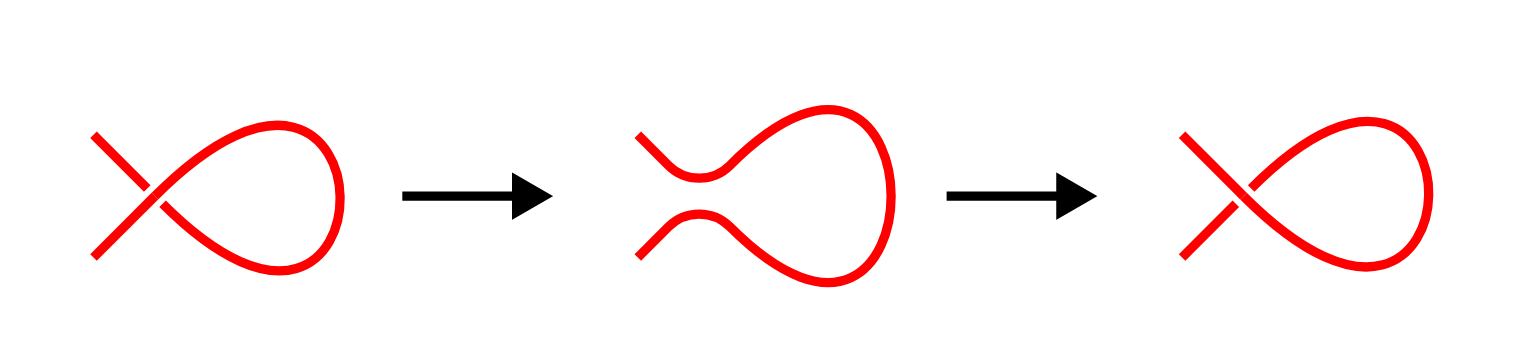
\includegraphics[width=50%,height=50%]{/home/vitalyr/projects/learn/Notebook/org/.attach/5c/a31ce0-780d-45d1-9bcf-1456d535bf9c/_20210529_165842screenshot.png}
\end{center}
\subsubsection{Definiton 2.2 Reidemeister move \(R2\)}
\label{sec:org638952b}
The second type of Reidemeister move, add or reduce a circle between two strand of line (locally) to a knot diagram, like this:
\begin{center}
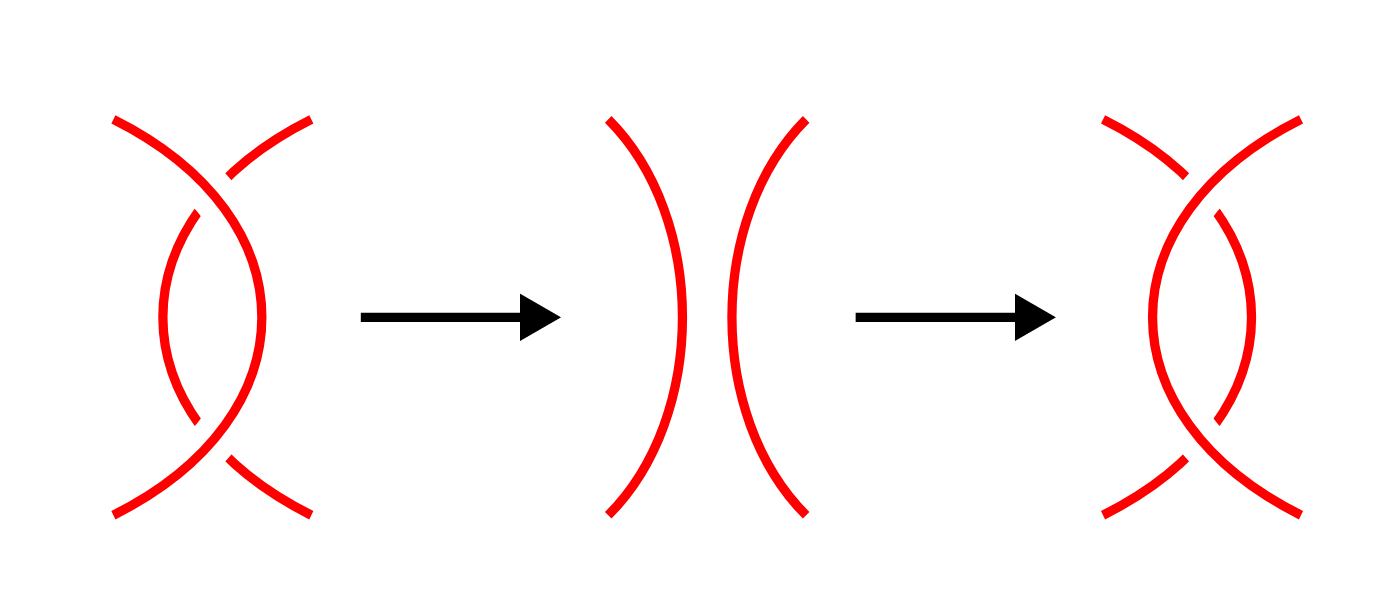
\includegraphics[width=50%,height=50%]{/home/vitalyr/projects/learn/Notebook/org/.attach/5c/a31ce0-780d-45d1-9bcf-1456d535bf9c/_20210529_170248screenshot.png}
\end{center}

\subsubsection{Definition 2.3 Reidemeister move \(R3\)\hfill{}\textsc{ATTACH}}
\label{sec:org35db08c}
The third type of Reidemeister move, move a  line over a crossing, or under a crossing, like this:
\begin{center}
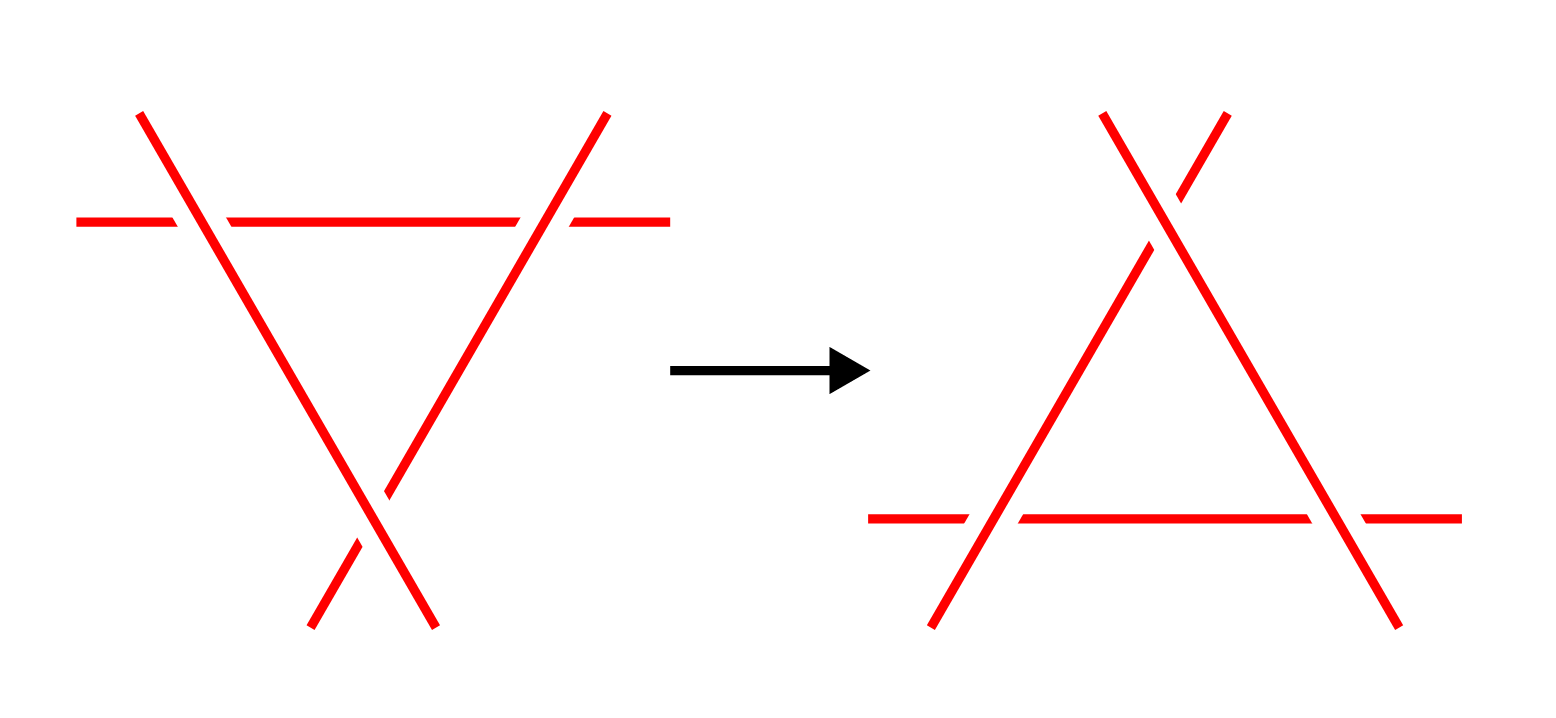
\includegraphics[width=50%,height=50%]{/home/vitalyr/projects/learn/Notebook/org/.attach/5c/a31ce0-780d-45d1-9bcf-1456d535bf9c/_20210529_170612screenshot.png}
\end{center}

No other part of the diagram is involved in the picture of a move, and a planar isotopy may distort the picture. The numbering for the types of moves corresponds to how many strands are involved, e.g. a type II move operates on two strands of the diagram.
One important context in which the Reidemeister moves appear is in defining knot invariants. By demonstrating a property of a knot diagram which is not changed when we apply any of the Reidemeister moves, an invariant is defined. Many important invariants can be defined in this way, including the Jones polynomial.
\subsection{Knot Invariants}
\label{sec:org3a7c8f2}
\subsubsection{The Jones Polynomial, HOMFLY-PT polynomial and Alexander polynomial}
\label{sec:org3a7b2ff}
The Jones Polynomial could be said to be the most important knot invariant so far. It is a special case of the HOMFLY-PT polynomial.
he HOMFLY-PT polynomial is a knot and link invariant.  Confusingly, there are several variants depending on exactly which relationships are used to define it.  All are related by simple substitutions
.
\begin{enumerate}
\item Definition
\label{sec:org7bfcc57}

To compute the HOMFLY-PT polynomial, one starts from an oriented link diagram and uses the following rules:

\begin{enumerate}
\item \(P\) is an isotopy invariant (thus, unchanged by Reidemeister moves).
\item \(P(\text{unknot}) = 1\)
\item Let \(L_+\), \(L_-\), and \(L_0\) be links which are the same except for one part where they differ according to the diagrams below.  Then, depending on the choice of variables:

\begin{enumerate}
\item \(l \cdot P(L_+) + l^{-1} \cdot P(L_-) + m \cdot P(L_0) = 0\).
\item \(a \cdot P(L_+) - a^{-1} \cdot P(L_-) = z \cdot P(L_0)\).  (Sometimes \(\nu\) is used instead of \(a\))
\item \(\alpha^{-1} \cdot P(L_+) - \alpha \cdot P(L_-) = z \cdot P(L_0)\).
\item Using \textbf{three} variables: \(x \cdot P(L_+) + y \cdot P(L_-) + z \cdot P(L_0) = 0\).
\end{enumerate}

\$\$
\begin{array}{ccc}
\begin{svg}[[!include SVG skein positive crossing]]\end{svg} &
\begin{svg}[[!include SVG skein negative crossing]]\end{svg} &
\begin{svg}[[!include SVG skein no crossing]]\end{svg} \\
L_+ & L_- & L_0
\end{array}
\$\$
\end{enumerate}

From the rules, one can read off the relationships between the different formulations:

\begin{enumerate}
\item \(y = \alpha = a^{-1}\)
\item \(x = - \alpha^{-1} = -a\)
\item \(a = - i l\), \(l = i a\)
\item \(z = i m, m = - i z\).
\end{enumerate}


\item Properties
\label{sec:orgb0817dd}

The HOMFLY polynomial generalises both the Jones polynomial and the Alexander polynomial.

\begin{enumerate}
\item To get the Jones polynomial, make one of the following substitutions:
\label{sec:orge7dcbb2}

\begin{enumerate}
\item \(a = q^{-1}\) and \(z = q^{1/2} - q^{-1/2}\)
\item \(\alpha = q\) and \(z = q^{1/2} - q^{-1/2}\)
\item \(l = i q^{-1}\) and \(m = i (q^{-1/2} - q^{1/2})\)
\end{enumerate}

\item To get the Alexander polynomial, make one of the following substitutions:
\label{sec:orgcee9fe8}

\begin{enumerate}
\item \(a = 1\), \(z = q^{1/2} - q^{-1/2}\)
\item \(\alpha = 1\), \(z = q^{1/2} - q^{-1/2}\)
\item \(l = i\), \(m = i (q^{-1/2} - q^{1/2})\)
\end{enumerate}
\end{enumerate}
\end{enumerate}
\subsubsection{The Unknotting number}
\label{sec:org179c1e7}
In the mathematical area of knot theory, the unknotting number of a knot is the minimum number of times the knot must be passed through itself (crossing switch) to untie it. If a knot has unknotting number n, then there exists a diagram of the knot which can be changed to unknot by switching n crossings.
If you had a piece of string possibly tangled up, and could, at a crossing, pull one part of the string through the other, then, intuitively, repeating this enough times, the string would become unknotted. At the mathematical level, there is a corresponding notion of a crossing change on a diagram.

\textbf{Definition}. A crossing change in a diagram exchanges an overpass and underpass at a crossing, as below:
<image>
(The central arrow should be a left-right arrow, but the arrowheads do not come out!)
Crossing changes will usually alter the isotopy type of the diagram.
\textbf{Lemma}. Let \(D\) be a diagram with \(c\) crossings, then changing at most \(c/2\) crossings of D produces a diagram of the unknot.
\textbf{Proof}. After changing a crossing of \(D\), we could reduce at lease one crossing with a R1 move.
\textbf{Definition}. The unknotting number, \(u(K)\), is the smallest number of crossing changes required to obtain the unknot from some diagram of the knot \(K\).

\subsection{Kanenobu Knot, Generalized Kanenobu Knot and Alternating Link\hfill{}\textsc{ATTACH}}
\label{sec:orga2c33f1}
The  Kanenobu Knots, which are infinitely many knots with the same knot ploynomial invariant, \cite{kanenobuInfinitelyManyKnots1986} , are knots like following:
:ID:       4f7bf60b-78ae-4365-b59d-29b51ce88612
\begin{center}
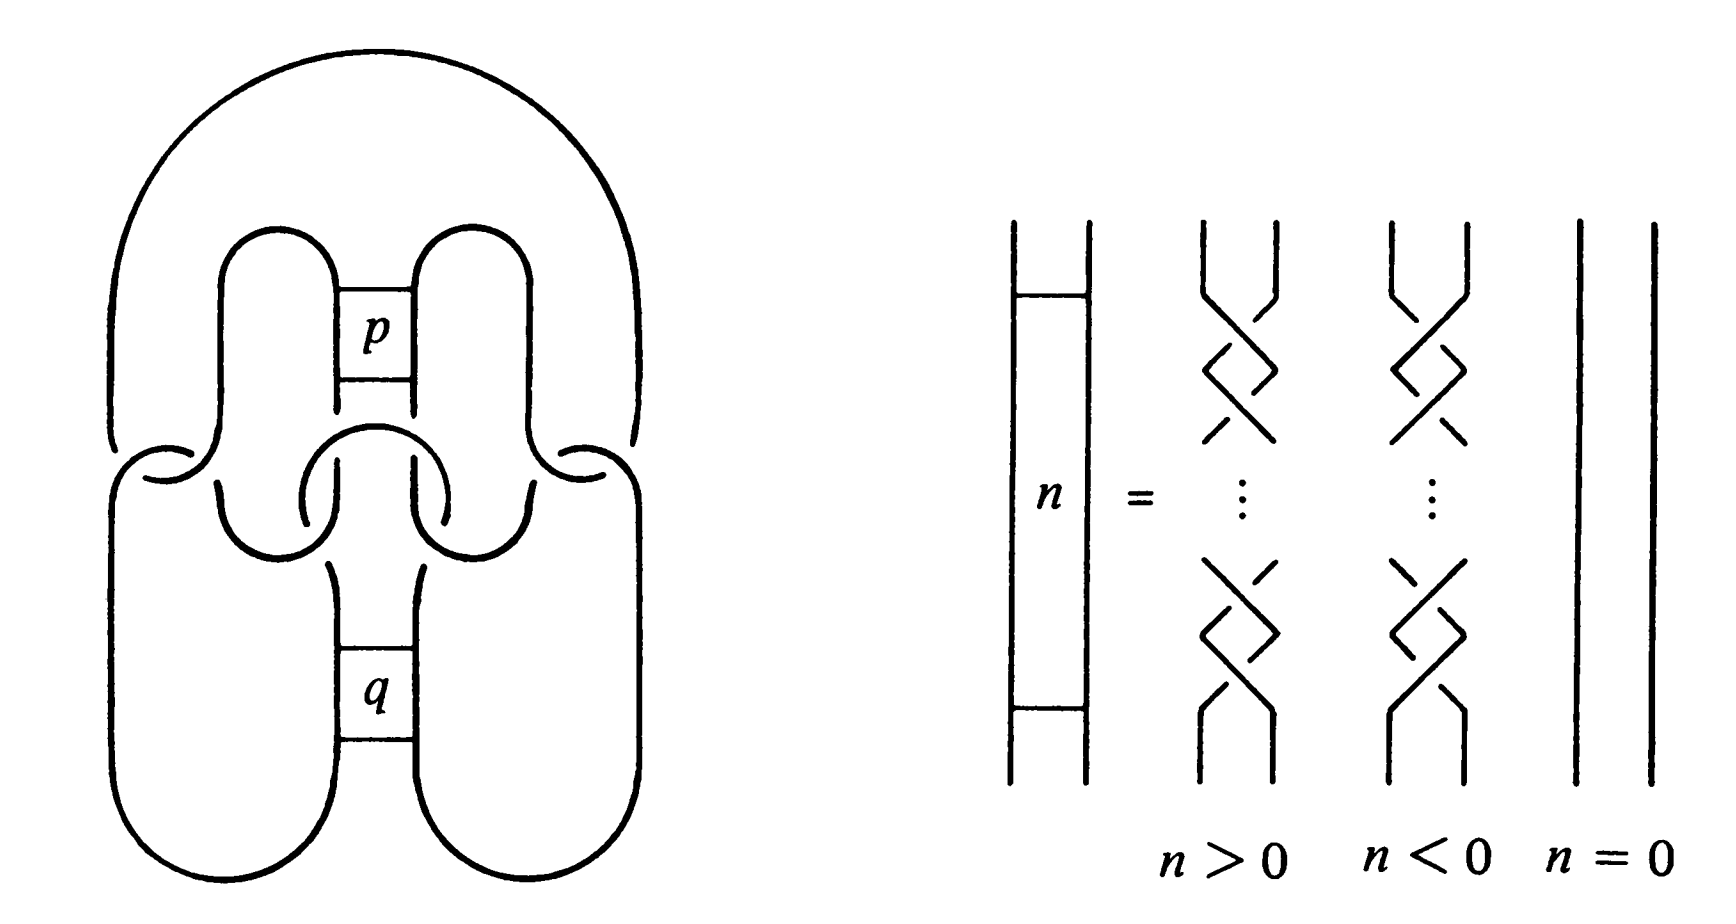
\includegraphics[width=50%,height=50%]{/home/vitalyr/projects/learn/Notebook/org/.attach/57/5a3ce3-c2d4-4d15-874f-4054cf3c0acc/_20210523_133107screenshot.png}
\end{center}

The Kanenobu knot with parameter p, q is represented  by K(p,q). When p>0, the upper braid  has the right curve above. When p<0, the upper braid has the left curve above. When q>0, then lower braid has the left curve above. The q<0, the lower braid has the left curve above.

\subsubsection{Generalized Kanenobu Knot\hfill{}\textsc{ATTACH}}
\label{sec:org60fe2ce}
The Kanenobu knot could be generalized by adding more parameters. After adding twisting between every crossing point of it, we get K(p, q, m, n):
\begin{center}
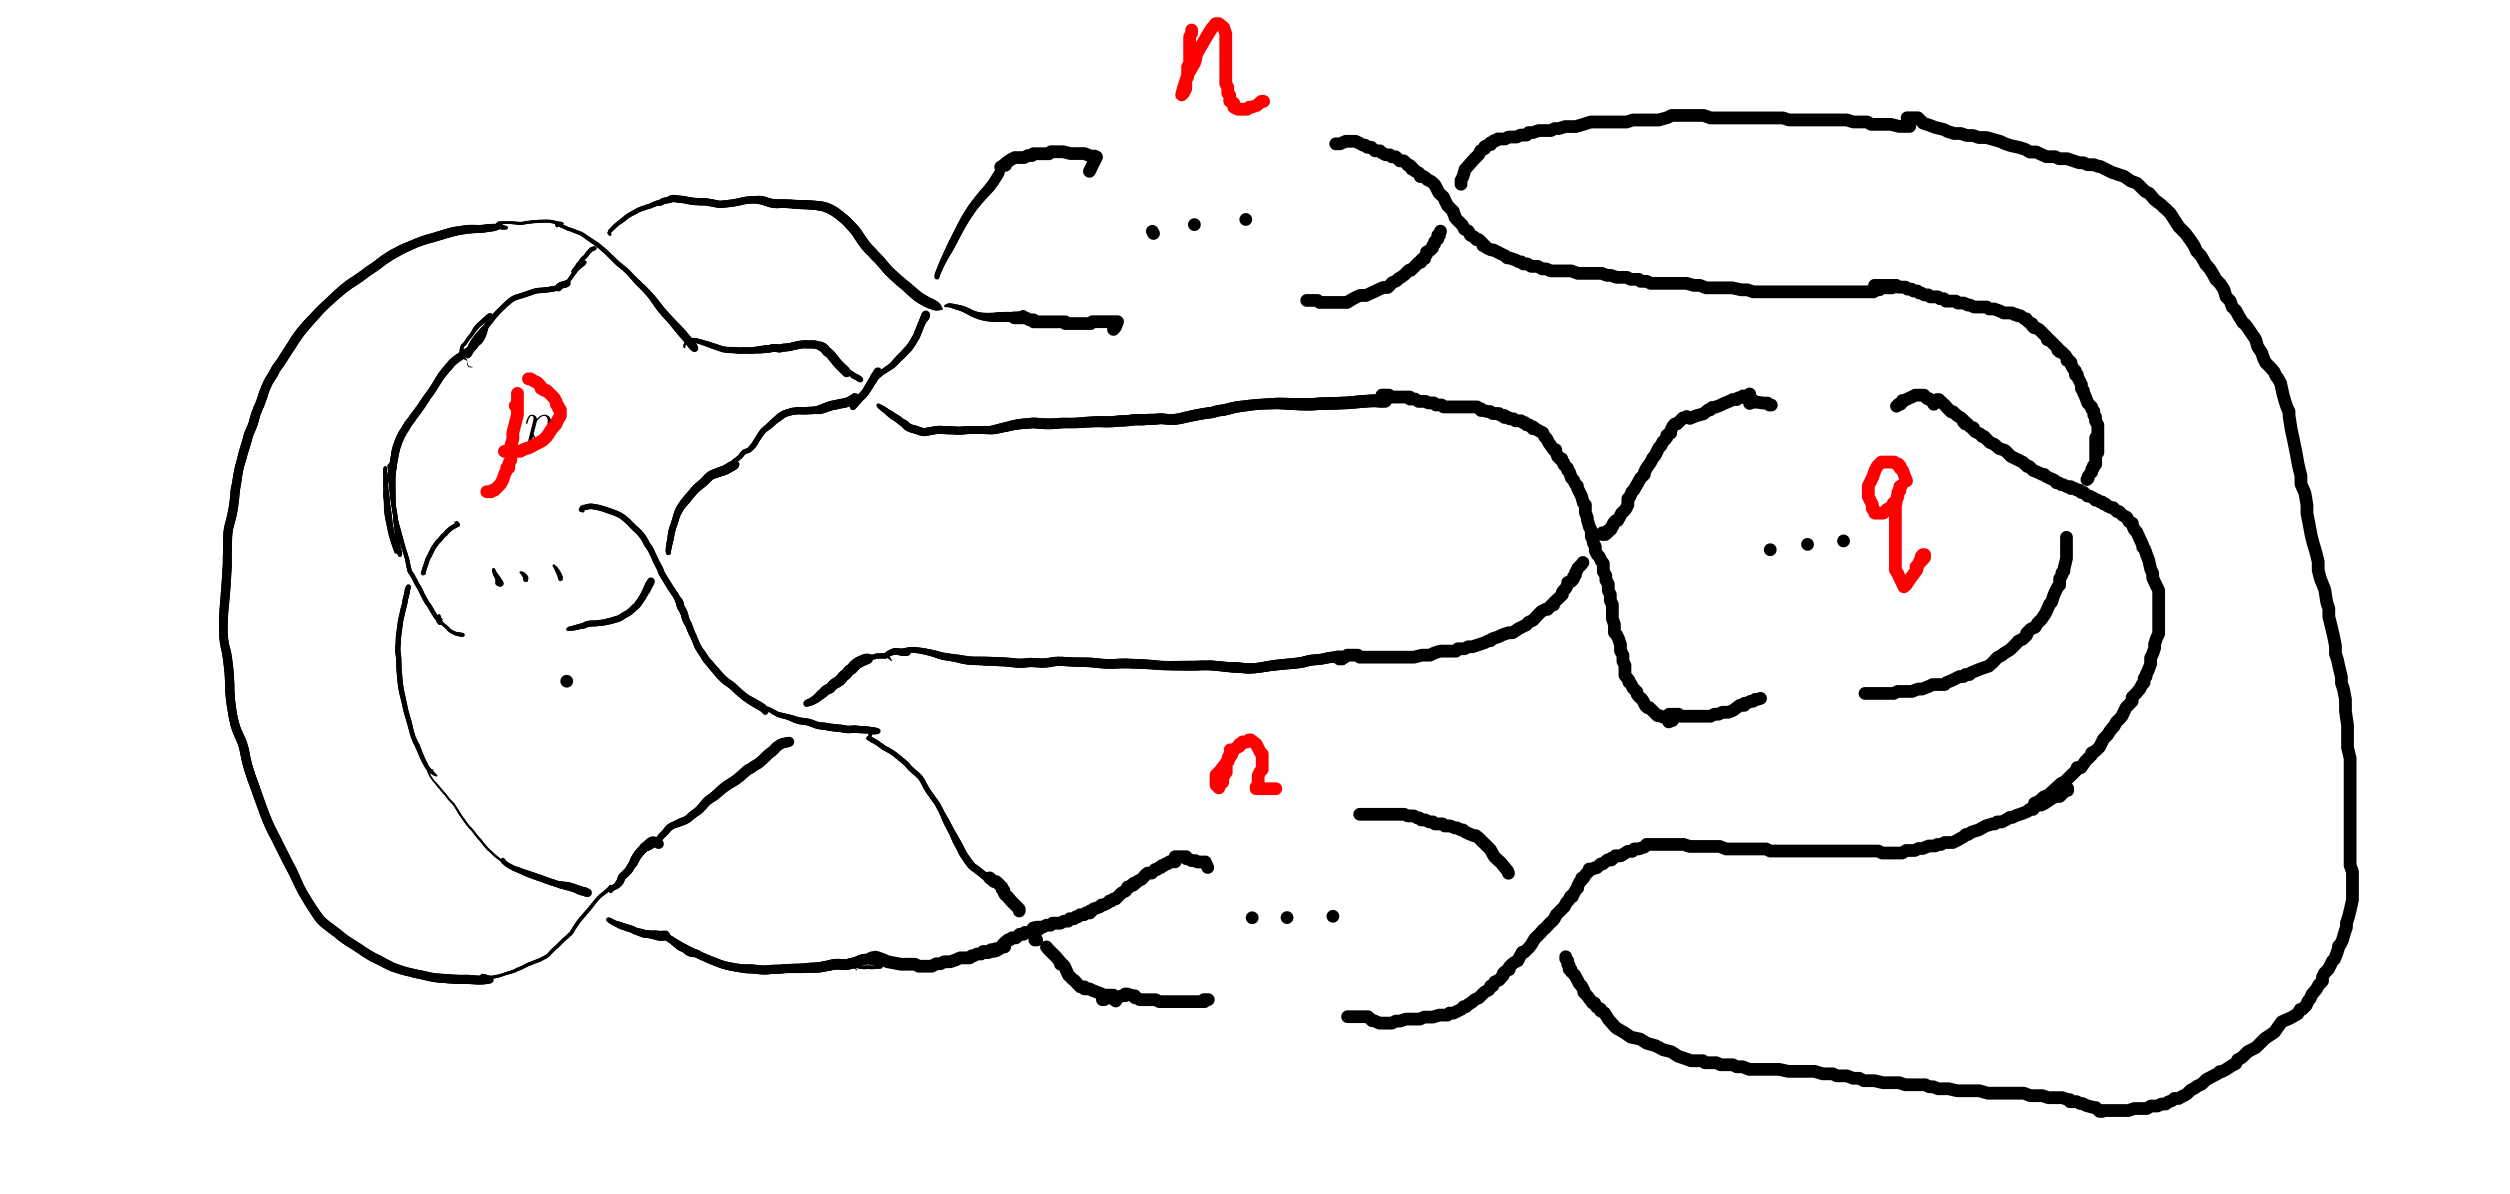
\includegraphics[width=50%,height=50%]{/home/vitalyr/projects/learn/Notebook/org/.attach/57/5a3ce3-c2d4-4d15-874f-4054cf3c0acc/_20210523_135628screenshot.png}
\end{center}

\cite{kanenobuInfinitelyManyKnots1986}
By adding parameters further, we get \(K(p, q, m, n, l\):
\begin{center}
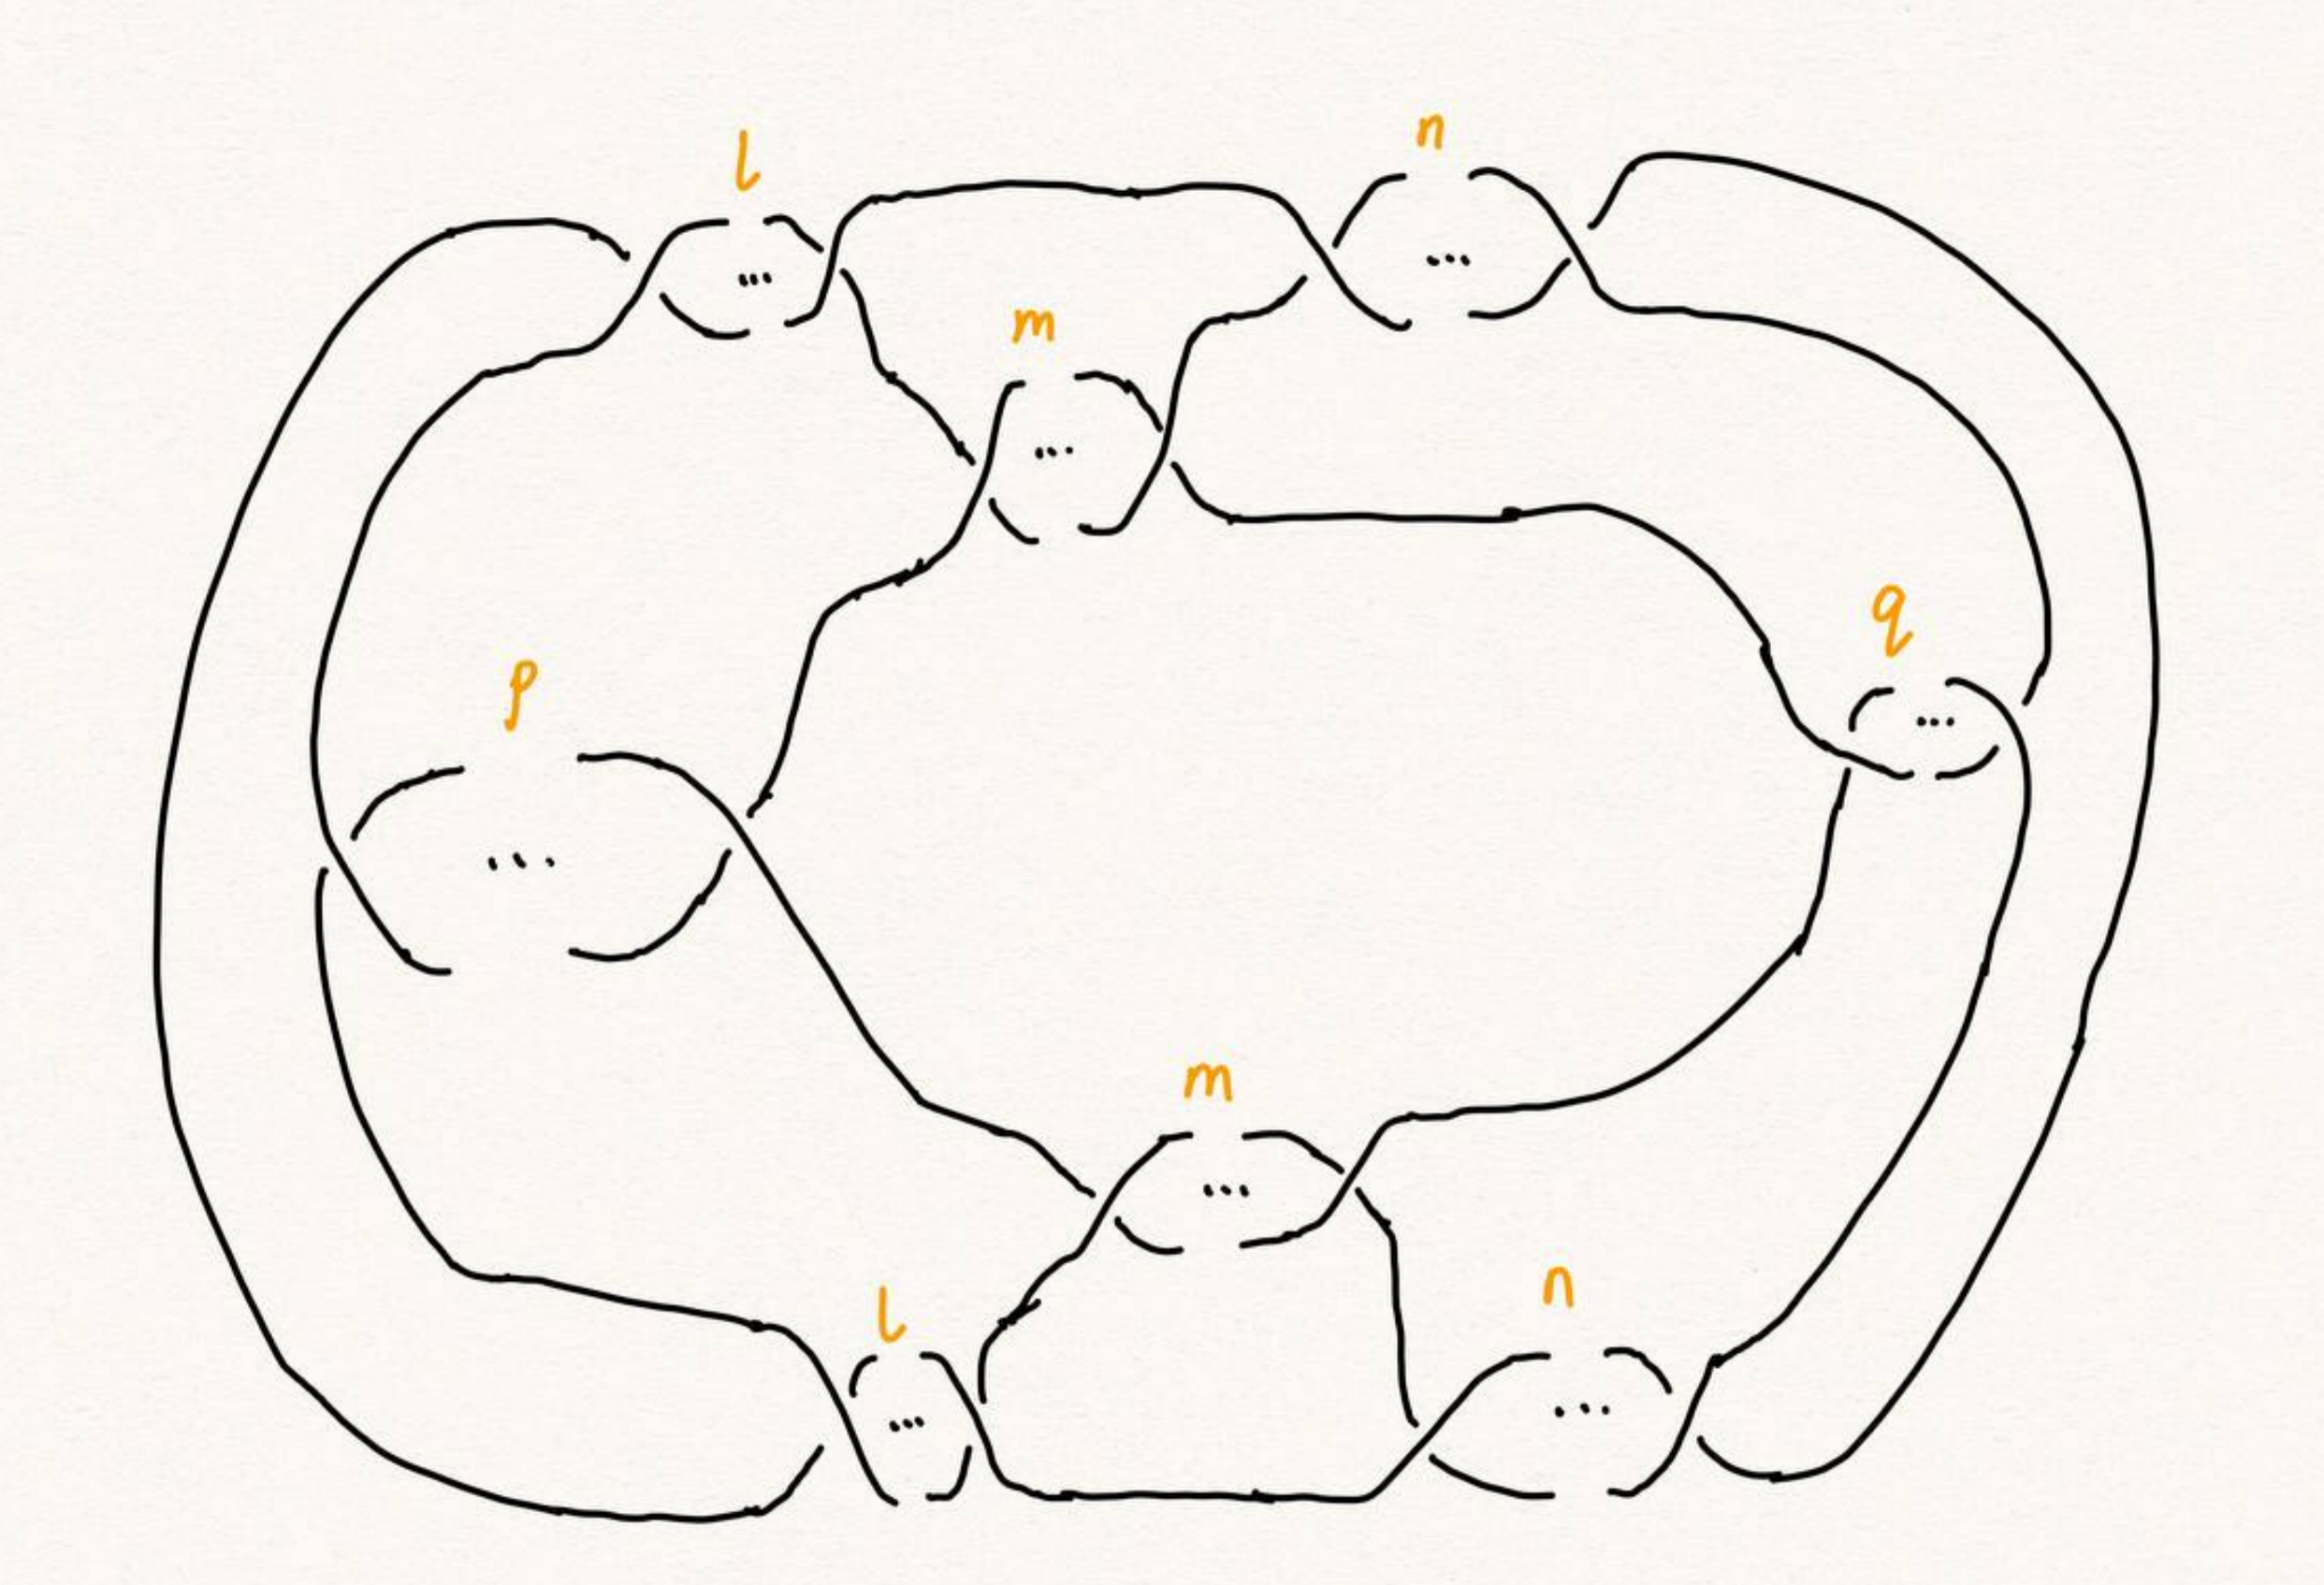
\includegraphics[width=.9\linewidth]{/home/vitalyr/projects/learn/Notebook/org/.attach/57/5a3ce3-c2d4-4d15-874f-4054cf3c0acc/_20210531_040613screenshot.png}
\end{center}
Which has all its crossing point be a crossing point family.
\subsubsection{Alternating Link}
\label{sec:org58507cf}
If in the diagram of a link, the crossings are alternating to each other, which means if one line in one crossing point is above, and in every neighbor crossing point it's below, we say this link is an alternating link.
\begin{center}
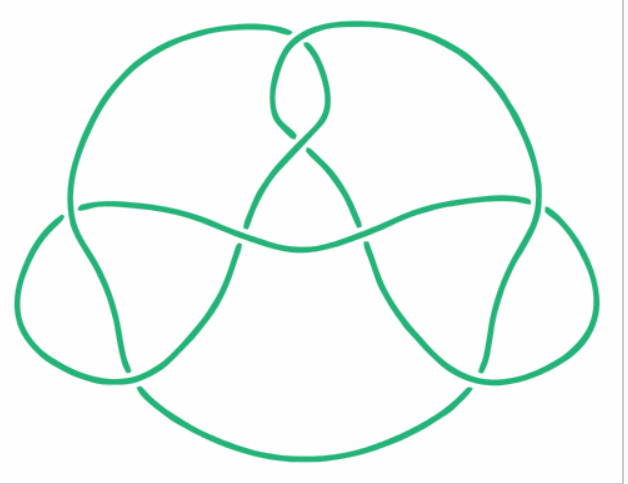
\includegraphics[width=50%,height=50%]{/home/vitalyr/projects/learn/Notebook/org/.attach/57/5a3ce3-c2d4-4d15-874f-4054cf3c0acc/_20210531_033544screenshot.png}
\end{center}

\section{Section 3. Unknotting Number for Kanenobu Knot}
\label{sec:org8b5031c}
This section we will investagate the unknotting number for Kanenobu Knot.
\subsection{Theorem 3.1 Every alternating link is not an unknot.}
\label{sec:org044022c}
\textbf{Proof} We can't change any crossing for every crossing point is alternating. To change one crossing, we could impact Reidemester move R1 or R2 on the link. With the property of alternating, we could reduce any crossing point, thus it can't be an unknot.
\subsection{Theorem 3.1: the unknotting number of Kanenobu knot K(0,0) is 2.}
\label{sec:org6706ac5}
\textbf{Proof} . When p = 0, q = 0, the Kanenobu knot is like:
<image>


And we label the crossing point with numbers 1, 2, \ldots{} , 8.
First, we show that after changing the crossing point 1 and 8, this Kanenobu knot K(0, 0) will be transformed into an unknot.
\begin{enumerate}
\item After changing 1 and 8, the knot becomes:
\end{enumerate}
<image>
\begin{enumerate}
\item Then we put a R2 move to the part between crossing point 1 and 2, and another R2 move to the part between crossing point 7 and 8, we get:

\item put a R2 move to the part between crossing point 4 and 5, we get:

\item put a R2 move to the part between crossing point 3 and 4, and another R2 move to the part between crossing point 5 and 6, we get the unknot.
\end{enumerate}

Second, we show that for any one change to the crossing point, the Kanenobu knot won't be transformed to the unknot.
\begin{enumerate}
\item If we change the crossing point 1, we get an alternating knot, and alternating knot is not an unknot:

\item If we change the crossing point 2, we get an alternating knot, and alternating knot is not an unknot:
\end{enumerate}
\ldots{}

All other circumstances could be applied to the same procedure. Thus the knot can't be untied by changing one crossing. Then we proved the unknotting number for Kanenobu knot K(0, 0) is 2.
\section{Section 4. Unknotting Number for Generalized Kanenobu Knot}
\label{sec:org6349c9d}
\subsection{Lemma 4.1 The Generalized Kanenobu knot is not an unknot.}
\label{sec:org2edf65b}
\textbf{Proof} From Theorem 5 in [9], we have assertion about the Khovanov homology for generalized Kanenobu knot:
\(Kh(K_{\beta}(p,q)) \cong K_{beta}(p+1, q-1)\) ,
then the genalized Kanenobu knot has different Khovanov homology with unknot, which mease it is not an unknot.
\subsection{Theorem 4.2 The unknotting number for Generalized Kanenobu knot K(p, q) is 2.}
\label{sec:org7402e51}
\textbf{Proof}.
Label the 12 crossing points (excluding the p, q, n crossing points) with number 1, 2, \ldots{}, 12.
First, change crossing points 2, 9, then  we could untie all the crossing point between 6 and 12.
We could untie all the crossing points between 4 and 5, 10 and 11. Thus the all the points
:ID:       23575a83-0649-48c0-ad07-54b2c55a79b9

Then we must prove changing points less than 2 we can not untie this knot.
If we changes 0 crossing point, this problem is trivial: the Kanenobu knot K(p, q, n) remains not an unknot.
If we changes only 1 crossing point:
<image>
\begin{enumerate}
\item if we change the crossing point 1, the part between is alternating and the whole knot is not an unknot.
\item if we change the crossing point 2, the knot will become:
<image>
\end{enumerate}
And it is not an unknot because we can not untie the twist in the \(n\) part, for locally it is alternating.

\begin{enumerate}
\item If we change any crossing point other than 1, 2, the situation are similar to thing above.
\end{enumerate}

Thus we can't untie the knot with only 1 crossing point change. Then we proved the unknotting number for generalized Kanenobu knot is 2.
\section{Section 5. Unknotting Number for More Generalized Kanenobu Knot}
\label{sec:org76bd4fd}
The more generalized Kanenobu knot is complex then we will break this problem into several situations.
First, we introduce plat form for a surface-link to help solve this problem.
\subsection{5.1 a plat form for a surface-link}
\label{sec:org3726b77}
\subsubsection{test image:}
\label{sec:org1d14dfc}
\url{https://gitee.com/Vitaly/img/raw/master/images/Pictures/anime/2021-10-05-15-05-31-20a0bded101e077be23a7ca35ed49b77-bf36.jpg}
In this section, we introduce a plat form for a surface-link.We assume \(D_{2}\subset \mathbb{R}^{2}\). Let \(N\) be a regular neighborhood of \(\partial D\) in \(\mathbb{R}^{2}\ Int D_{2}\), which is parameterized with \((t, x) \in * \times S^{1}\) such that \(\partial D_{2} ={0} \times S^{1}\) and \(y_{0}=(0,0) \in * \times S^{1}\), where \(S^{1} =\mathbb{R}/\mathbb{Z}\).
\begin{center}
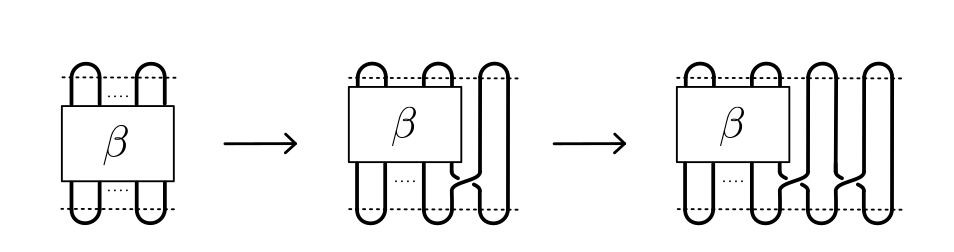
\includegraphics[width=50%,height=50%]{/home/vitalyr/projects/learn/Notebook/org/_20210524_052044screenshot.png}
\end{center}
\subsubsection{Definition 5.1.1 A surface A in \(D_{1} \times N\) is of m-wicket type (or simply of wicket type) if it is a properly embeded surface in \(D_{1} \times N\) satisfying the following conditions.}
\label{sec:org92f5658}
(1) \(A \cap D_{1} \times (I \times {0})\) is the standard m-wicket system when we identify \(D_{1} \times (I \times {0})\) with \(D \times [0,1]\).
(2) For each \(\theta \in S^{1}\),\(A \cap (D_{1}\times (*I \times {\theta}))\) is an m-wicket system.

Definition 5.1.2 A braided surface \(S\) in \(D_{1} \times D_{2}\) is adequate if there exists a surface of m-wicket type, \(A\), in \(D_{1} \times N\) such that the boundaries of S and A coincide: \(\partial S = \partial A\).

It's tivial that the degree of an adequate braided surface is even. Note that for each \(\theta \in S^{1}\), the seciton \(A \cap  D_{1} \times (*I \times {\theta})\)  is determined from the boundary of A and hence A is determined by \(\partial S\). Therefore, for an adequate braided surface \(S\), such a surface A of wicket is uniquely determined.

We consider a condition for a braided surface to admit the plat closure. For a
braided surface \(S\) of degree n, let \(\beta_{S}\) be a geometric \(n\)-braided obtained by cutting the closed braid \(\partial S\) along \(\pi ^{-1}(y_{0})\). It is easy to say that \([\beta_{S}] = [\beta_{S^{'}}]\) in the braided group \(B_{n}\) if two braided surfaces \(S\) and \(S'\) are equivalent.
\subsubsection{Theorem 5.1.2 A braided surface \(S\) is equivalent to an adequate one if and only if \({\rm deg} S = 2m\) for some \(m \in \mathbb{N}\) and the braid \([\beta_{S}]\) belongs to \(K_{2m}\).}
\label{sec:org3ef03e2}
\textbf{Proof} . Let \(S\) be equivalent to an adequate braided surface \(S_{0}\), and let \(A_{0}\) be a surface of \(m\)-wrick type such that \(\partial S_{0} = \partial A_{0}\). Thus \({\rm deg} S = {\rm deg } S_{0} = 2m\) for some \(m \in \mathbb{N}\), and \([\beta_{S}]=[\beta_{S_{0}}]\). Let \(f:[0,1] -> \mathscr{W}_{m}\) be a map defined by \(f(t) = A_{0} \cap D_{1} \times (I \times {t})\). Then \(f\) is a loop in \(\mathscr{W}_{m}\)such that \(f(0) = f(1)\) is the standard m-wicket system. By the isomorphism, the element \([f] \in \mathscr{W}_{m}\) corresponds to the braid \([\beta_{f}] \in K_{2m}\). Since \(\partial S_{0} = \partial A_{0}\), we have \(\beta_{S_{0}} = \beta_{f}\). Thus, \(\beta_{S} \in K_{2m}\).

The more generalized Kanenobu knot \(K(p, q, l, m, n\)is like:

<image>

\subsection{Theorem 5.1 The unknotting number for more generalized Kanenobu knot \(K(p, q, m, n, l)\) is:}
\label{sec:org8798504}

\subsubsection{When \(n>m\), the unknotting number for \(K(p, q, m, n, l)\) is \(2[\frac{n+l}{2}]\), where \([\frac{n+l}{2}]\) is the integer part of \(\frac{n+l}{2}\)\hfill{}\textsc{ATTACH}}
\label{sec:org73e7558}

\subsubsection{When \(m>n\), the unknotting number for \(K(p, q, m, n, l)\) is \(2[\frac{m+l}{2}]\), where \([\frac{m +l}{2}]\) is the integer part of \(\frac{m +l}{2}\)}
\label{sec:org9fed131}
\subsubsection{When \(q + n < m + l\) and \(q + n < n + l\), the unknotting number for \(K(p, q, m, n, l)\) is \(2[\frac{q+n}{2}]\), where \([\frac{q+n}{2}]\) is the integer part of \(\frac{n+l}{2}\).}
\label{sec:org997889b}

\textbf{Proof}. First we should show that with the numbers of crossing point changes, we can untie the knot.
When \(m>n\), after changes the crossing points in the \(m\) and \(l\) part (do this by reduing \([\frac{m+l}{2}]\) crossing points), we get the knot like:

<image>
We can untie this knot by twisting the \(q\) crossing numbers first, then the 2 \(n\) crossing points.

When \(n>m\), after changing the crossing points in \(n\) and \(l\) part(do this by reducing \([\frac{n+l}{2}]\) crossing numbers), we get the knot like:
<image>
We can untie this knot by reducing the \(p\) part first, then \(l\) part.

When \(q + n < m + l\) and \(q + n < n + l\), we would untie the \(q\) and \(n\) part with \(2[\frac{q+n}{2}]\) changes, and get this:
<image>
Then we could untie the whole knot.

Second, we must show we can not untie this knot with any other ways.
With theorem 5.1.2, the \(m , l\) braid has the same plat form with the \(n, l\) part, they are the only two ways to untie this knot. This completes this proof.

\section{Section 6. Acknowledgements}
\label{sec:orga9959b7}
 After more than five months of  work, I finally finished writing my thesis. During this time, I learned a lot and felt a lot. From knowing nothing, I read books of Professor Jiang, and GTM series. I look up every concept from various source: wikipedia, The KnotBook, etc. Every time I understood a new concept and new theorem was the gain of my study, and every successful proof of a theorem would make me happy for a few days.

My thesis is not very mature. It only deal with a simple situation of a special kind of knot. But this experience of doing my dissertation has benefited me for life. I feel that doing a dissertation is something that you really have to put your heart and soul into, it is truly a process of learning and researching on your own, otherwise it will not be called a dissertation.

June, it's always sunny. In June, it's always the end of the song. In June, we refuse to be sentimental. The flowers give up their fragrance and we welcome the fruits. Graduation brings farewell, and we are on our way to glory. As I finish my thesis, I want to express my deepest gratitude to my supervisor and my dear family! I would like to thank my supervisor, Ms. Wan. She has been a role model for me, a trusted mentor and friend, both as a person and in her studies. She cares about my study and research. From choosing a topic for my dissertation, writing the opening report, searching for information, to writing thesis, she gave me  useful guidance so that I could successfully complete my dissertation. She also often supervised and motivated the lazy me to finish my characters on time. Thank you, Ms Wan!

In addition, I would like to thank to the Jike App, I had a group of online interesting friends to keep me company while I was writing the thesis. I would like to thank the Rust programming language which is elegant and powerful to write my toy projects. I would like to thank the Veloren game, which is a free voxel game and is developed in the Rust programming language. It is so relaxing where staying at the game world. I used Emacs and org-mode to produce all my papers, and then used Microsoft Word to format them according to the university's requirements. Thanks to the creator of GNU Emacs, Richard M. Stallman, the creator of org-mode Dominik and the current maintainer Bastien Guerry, and to everyone in the Emacs community.

\subsection{[1] S.Fukuhara, Y.Matsumoto, O.Saeki, An estimate for the unknotting numbers of torus knots[J], Topology and its Applications, 1991, 38(3): 293-299}
\label{sec:org2681f4a}
\subsection{[2] 姜伯驹,绳圈的数学,湖南教育出版社[M],1991}
\label{sec:orga81bc1c}
\subsection{[3] B. Owens, On slicing invariants of knots[J], Journal of Knot Theory and Its Ramifications, 2011, 14(01):3-8.}
\label{sec:org9da4c73}
\subsection{[4] V.Siwach, P. Madeti, Unknotting Number of Some Knots[J], Elsevier, 2014}
\label{sec:org71630ce}
\subsection{[5] V. Siwach, M. Prabhakar, A Method for Unknotting Torus Knots[J], Mathematics, 2012}
\label{sec:orga6bf995}
\subsection{[6] Rolfen, Knots and Links[M], Publish or Perish, 1976}
\label{sec:orgbbdadd4}
\subsection{[7] W.B. Raymond Lickorish, Introduction to Knot Theory[M], Springer, 1997}
\label{sec:org8bf07f7}
\subsection{[8] C.C. Adams, The Knot Book: An Elementary Introduction to the Mathematical Theory of Knots[M], W.H.Freeman and Company, New York, 1994}
\label{sec:org2f41126}
\subsection{[9] Kanenobu, T., Infinitely Many Knots with the Same Polynomial Invariant, Proceedings of the American Mathematical Society, 97(1), 158–162 (1986).  \url{http://dx.doi.org/10.2307/2046099}}
\label{sec:org33355f0}

\cite{kanenobuInfinitelyManyKnots1986}

\bibliographystyle{apacite}
\bibliography{library}
\end{document}
